\documentclass[11pt,oneside]{article}
\usepackage[utf8]{inputenc}
\usepackage[a4paper,top=2cm,left=2cm,right=2cm,bottom=2cm]{geometry}
\usepackage{import}
\usepackage[T1]{fontenc}
\usepackage[german,ngerman]{babel}
\usepackage[table]{xcolor}
\usepackage{amsthm, esvect}
\usepackage{mathtools}
\RequirePackage{amssymb, amsfonts, amsmath, latexsym, verbatim, xspace}
\usepackage{systeme}
\usepackage{multicol}
\usepackage{multirow}
\usepackage{framed}
\usepackage{array}
\usepackage{ragged2e}
\usepackage{graphicx}
\usepackage{pdflscape}
\usepackage{epstopdf}
\usepackage{booktabs}
\usepackage{pdfpages}
\usepackage{float} % Allows putting an [H] in \begin{figure} to specify the exact location of the figure
\usepackage{wrapfig} % Allows in-line images such as the example fish picture
\usepackage{tikz, graphicx} % tikz
\usepackage[position=top]{subfig}
\usepackage[bookmarks=true]{hyperref}%Links
\usepackage{enumerate}
\usepackage{enumitem}
\usepackage[german,ruled,vlined,linesnumbered,algosection]{algorithm2e}
\usepackage[labelfont=sf]{caption}
\usepackage{lmodern}
\usepackage{lscape}
\usepackage{tabularx}
\usepackage{systeme}
\usepackage{hhline}
\usepackage{subfiles}
\usepackage{stackengine}
\usepackage{setspace}
\usepackage{MnSymbol}
\usepackage{tcolorbox}
\usepackage{bbm}
\usepackage{url}
\usepackage{xparse}
\usepackage{sectsty}
\usepackage{array}
\usepackage{ragged2e}
\usepackage{listings} %Stellt Code-Snippets sauber dar

% definiert die Sprache
\selectlanguage{German}

% add command for different dates in Swiss fashion
\newcommand{\monthwordlong}[1]{\ifcase#1 \or Januar\or Februar\or März\or April\or Mai\or Juni\or Juli\or August\or September\or Oktober\or November\or Dezember\fi}
\newcommand{\monthwordshort}[1]{\ifcase#1\or Jan\or Feb\or Mar\or Apr\or Mai\or Jun\or Jul\or Aug\or Sept\or Okt\or Nov\or Dez\fi}
\newcommand{\datelong}{\number\day.\:\monthwordlong{\the\month}\:\number\year}
\newcommand{\dateshort}{\number\day.\:\monthwordshort{\the\month}\:\number\year}

% define color of links inside a text
\definecolor{linkblue}{RGB}{0, 0, 80}
\definecolor{plotblue}{RGB}{100, 100, 255}
\definecolor{myblue}{RGB}{8,164,214}
\definecolor{myred}{RGB}{143,42,41}
\definecolor{forestgreen}{RGB}{34,139,34}
\definecolor{highdive}{RGB}{10,169,194}
\definecolor{charcoal}{RGB}{74,74,74}
\hypersetup{
	colorlinks=true,
	linkcolor=linkblue,
	filecolor=magenta,
	urlcolor=plotblue,
	citecolor=linkblue,
	pdfpagemode=FullScreen,
}


\lstdefinestyle{mystyle}{ % definiert den style des Code-Snippets
	%backgroundcolor=\color{backcolour},
	%commentstyle=\color{codegreen},
	%keywordstyle=\color{magenta},
	%numberstyle=\tiny\color{codegray},
	%stringstyle=\color{codepurple},
	basicstyle=\ttfamily\footnotesize,
	breakatwhitespace=false,
	breaklines=true,
	captionpos=b,
	keepspaces=true,
	%numbers=left,
	%numbersep=5pt,
	showspaces=false,
	showstringspaces=false,
	showtabs=false,
	tabsize=4
}
\lstset{style=mystyle}
\usepackage{fancyhdr}

\tcbuselibrary{breakable,skins}
\usetikzlibrary{mindmap,trees}
\newlength\tindent
\setlength{\tindent}{\parindent}
\setlength{\parindent}{0pt}
\renewcommand{\indent}{\hspace*{\tindent}}

\makeatletter
\def\ifEmpty#1{\def\@temp{#1}\ifx\@temp\@empty}
\makeatother

\sectionfont{\underline}
\usetikzlibrary{arrows, petri, topaths, graphs}


% =================== BEISPIEL ====================
\theoremstyle{definition}
\newtheorem{beispiel}{Beispiel}
\renewcommand{\thebeispiel}{\arabic{beispiel}}

% =================== AUFGABE =====================
\newcounter{aufg}[section] % Zähler für die Umgebungen

\newenvironment{aufgabe}[1][]{%
    \refstepcounter{aufg}% Inkrementiere den Zähler
    \begin{tcolorbox}[%
        enhanced,
        overlay unbroken and first={\mytitleaufg[#1]}, % Titelleiste mit Icons wird nicht über Seite gebrochen
        colframe=black,
        boxrule=0pt,
        breakable,
        top=15pt,
        before=\vskip18pt,
    ]
}{%
    \end{tcolorbox}
}

\newcommand{\mytitleaufg}[1][]{% Definiert die Titelleiste und Icons
    \node[fill=black!20,
        rounded corners,
        draw=black,
        text=black,
        line width=1pt,
        inner sep=4pt,
        anchor=west,
        xshift=12pt]
        at (frame.north west){\bfseries Aufgabe \thesection.\theaufg.\ifEmpty{#1}\else\emph{ (#1)}\fi}; % Titel, letzter Teil mit ifempty testet ob #1 leer und macht Klammern und Titel, falls Titelargument übergeben wird bzw. falls #1 leer erscheint nichts - auch keine Klammern

    \node[% Icon
        rounded corners,
        text=black,
        fill=black,
        line width=0pt,
        inner sep=3pt,
        anchor=west,
        xshift=5pt,
        % yshift=-35pt
        ]
        at (frame.north east){
\includegraphics[width=24pt]{../../../Header/Icons/aufgabeicon.png}};
}

% =================== DEFINITION ==================
\newcounter{def}[section] % Zähler für die Umgebungen

\newenvironment{definition}[1][]{%
    \refstepcounter{def}% Inkrementiere den Zähler
    \begin{tcolorbox}[%
        enhanced,
        drop shadow southeast,
        overlay unbroken and first={\mytitledef[#1]}, % Titelleiste mit Icons wird nicht über Seite gebrochen
        colback=blue!5!white,
        colframe=blue!75!black,
        boxrule=2pt,
        breakable,
        top=15pt,
        before=\vskip18pt,
    ]
}{%
    \end{tcolorbox}
}

\newcommand{\mytitledef}[1][]{% Definiert die Titelleiste und Icons
    \node[fill=blue!40!white,
        rounded corners,
        draw=black,
        text=black,
        line width=1pt,
        inner sep=4pt,
        anchor=west,
        xshift=12pt]
        at (frame.north west){\bfseries Definition \thesection.\thedef.\ifEmpty{#1}\else\emph{ (#1)}\fi}; % Titel, letzter Teil mit ifempty testet ob #1 leer und macht Klammern und Titel, falls Titelargument übergeben wird bzw. falls #1 leer erscheint nichts - auch keine Klammern

    \node[% Icon
        rounded corners,
        text=black,
        fill=black,
        line width=0pt,
        inner sep=3pt,
        anchor=west,
        xshift=5pt,
        % yshift=-35pt
        ]
        at (frame.north east){
\includegraphics[width=24pt]{../../../Header/Icons/definitionicon.png}};
}

% =================== NOTATION ====================
\newcounter{nota}[section] % Zähler für die Umgebungen

\newenvironment{notation}[1][]{%
    \refstepcounter{nota}% Inkrementiere den Zähler
    \begin{tcolorbox}[%
        enhanced,
        drop shadow southeast,
        colback=yellow!5!white,
        colframe=yellow!75!black,
        overlay unbroken and first={\mytitlenota[#1]},   % Titelleiste mit Icons wird nicht über Seite gebrochen
        boxrule=2pt,
        breakable,
        top=15pt,
        before=\vskip18pt,
    ]
}{%
    \end{tcolorbox}
}

\newcommand{\mytitlenota}[1][]{% Definiert die Titelleiste und Icons
    \node[fill=yellow!40!white,,
        rounded corners,
        draw=black,
        text=black,
        line width=1pt,
        inner sep=4pt,
        anchor=west,
        xshift=12pt]
        at (frame.north west){\bfseries Notation \thesection.\thenota.\ifEmpty{#1}\else\emph{ (#1)}\fi}; % Titel, letzter Teil mit ifempty testet ob #1 leer und macht Klammern und Titel, falls Titelargument übergeben wird bzw. falls #1 leer erscheint nichts - auch keine Klammern

    \node[% Icon
        rounded corners,
        text=black,
        fill=black,
        line width=0pt,
        inner sep=3pt,
        anchor=west,
        xshift=5pt,
        % yshift=-35pt
        ]
        at (frame.north east){
\includegraphics[width=24pt]{../../../Header/Icons/definitionicon.png}};
}

% =================== SATZ ========================
\newcounter{satz}[section]  % creates a counter and resets it after each chapter

\newenvironment{satz}[1][]{   % Hauptbox mit Satz drin
    \refstepcounter{satz}
    \begin{tcolorbox}[%
        enhanced,
        colback=red!5!white,
        fuzzy halo=2mm with gray,
        colframe=red!75!black,
        overlay unbroken and first={\mytitlesatz[#1]},   % Titelleiste mit Icons wird nicht über Seite gebrochen
        boxrule=2pt,
        breakable,
        top=15pt,
        before=\vskip18pt,
    ]
}{%
    \end{tcolorbox}
}

\newcommand{\mytitlesatz}[1][]{                     % Macht Titelbox und Icons
   \node[fill=red!90!white,
      rounded corners,
      draw=black,,
      text=black,
      line width=1pt,
      inner sep=4pt,
      anchor=west,
      xshift=12pt]
   at (frame.north west){\bfseries Satz \thesection.\thesatz.\ifEmpty{#1}\else\emph{ (#1)}\fi};  % Titel, letzter Teil mit ifx testet ob #1 leer und macht Klammern und Titel, falls Titelargument übergeben wird bzw.  falls #1 leer erscheint nichts - auch keine Klammern

 \node[ % Icon
      rounded corners,
      text=black,
      fill=black,
      line width=0pt,
      inner sep=3pt,
      anchor=west,
      xshift=5pt,
%     yshift=-35pt
]
   at (frame.north east){ 
\includegraphics[width=24pt]{../../../Header/Icons/satzicon.png} };
}

% =================== BEWEIS ======================
\newenvironment{beweis}[1][]{
    \begin{tcolorbox}[
        enhanced,
        overlay unbroken and first={\mybeweis[#1]},     % Titelleiste mit Icons wird nicht über Seite gebrochen
        colback=white,
        colframe=black,
        boxrule=0pt,
        breakable,
        top=15pt,
        before=\vskip18pt,
    ]
}{
        \end{tcolorbox}
}

\newcommand{\mybeweis}[1][]{                     % Macht Titelbox und Icons
   \node[fill=white,
      rounded corners,
      draw=black,
      text=black,
      line width=1pt,
      inner sep=4pt,
      anchor=west,
      xshift=12pt]
   at (frame.north west){\bfseries Beweis \ifEmpty{#1}\else\emph{ (#1)}\fi};  % Titel, letzter Teil mit ifx testet ob #1 leer und macht Klammern und Titel, falls Titelargument übergeben wird bzw.  falls #1 leer erscheint nichts - auch keine Klammern
}

% =================== ALGORITHM ===================
\newcounter{algo}[section]  % creates a counter and resets it after each chapter

\newenvironment{algo}[1][]{   % Hauptbox mit Satz drin
    \refstepcounter{algo}
    \begin{tcolorbox}[%
        enhanced,
        drop shadow southeast,
        colback=yellow!5!white,
        colframe=yellow!75!black,
        overlay unbroken and first={\algotitle[#1]},   % Titelleiste mit Icons wird nicht über Seite gebrochen
        boxrule=2pt,
        breakable,
        top=15pt,
        before=\vskip18pt,
    ]
}{%
    \end{tcolorbox}
}

\newcommand{\algotitle}[1][]{                     % Macht Titelbox und Icons
   \node[fill=yellow!40!white,
      rounded corners,
      draw=black,
      text=black,
      line width=1pt,
      inner sep=4pt,
      anchor=west,
      xshift=12pt]
   at (frame.north west){\bfseries \ifEmpty{#1}{Ablauf}\else{#1}\fi};  % Titel, letzter Teil mit ifx testet ob #1 leer und macht Klammern und Titel, falls Titelargument übergeben wird bzw.  falls #1 leer erscheint nichts - auch keine Klammern

 \node[ % Icon
      rounded corners,
      text=black,
      fill=black,
      line width=0pt,
      inner sep=3pt,
      anchor=west,
      xshift=5pt
      % yshift=-35pt
      ]
   at (frame.north east){ 
\includegraphics[width=24pt]{../../../Header/Icons/algoicon.png} };
}

% ================ Nummerierte Multicol ================
\newenvironment{enumcols}[1][]{
    \begin{enumerate}[label=\alph*)]\begin{multicols}{#1}
}{
    \end{multicols}\end{enumerate}
}



% =================================================
\usetikzlibrary{shapes,arrows}
\tikzstyle{decision} = [diamond, draw, fill=blue!20,
    text width=6em, text badly centered, node distance=4cm, inner sep=0pt]
\tikzstyle{block} = [rectangle, draw, fill=blue!20,
    text width=8em, text centered, rounded corners, minimum height=4em]
\tikzstyle{line} = [draw, -latex']
\tikzstyle{cloud} = [draw, ellipse,fill=red!20, node distance=2cm,
    minimum height=2em]

% Karriertes Papier für Antwort
\newcommand{\karos}[1]{\begin{tikzpicture}\draw[step=0.5cm,color=gray] (0,0) grid (\linewidth,#1 cm);\end{tikzpicture}}
%%
% Header and Footer
%%
\linespread{1.2} % Line spacing
\fancypagestyle{plain}{
	\pagestyle{fancy}
	\lhead{}
	\chead{}
	\rhead{}
	\lfoot{\Autor}
	\cfoot{\Skriptname}
	\rfoot{\thepage}
	\renewcommand{\headrulewidth}{0pt}
	\renewcommand{\footrulewidth}{0.4pt}
}

\pagestyle{fancy}
\fancyhf{}
\rhead{\rightmark}
\lfoot{\leftmark}
\rfoot{\thepage}
\renewcommand{\headrulewidth}{0.2pt}
%\setlength\parindent{0pt} % Uncomment to remove all indentation from paragraphs



%%
% Math Arrows
%%
\newcommand{\same}{\ensuremath{\Longleftrightarrow}}
\renewcommand{\to}{\ensuremath{\longrightarrow}}
\newcommand{\qsame}{\quad\same\quad}
\newcommand{\dsame}{\ensuremath{:\Leftrightarrow}}
\newcommand{\qdsame}{\quad\dsame\quad}
\newcommand{\ldsame}{\ensuremath{:\Longleftrightarrow}}
\newcommand{\samedef}{\ensuremath{\us {\text{def}} \Leftrightarrow}}
\newcommand{\qsamedef}{\quad\samedef\quad}
\newcommand{\lsamedef}{\ensuremath{\us {\text{def}} \Longleftrightarrow}}
\newcommand{\qlsamedef}{\quad\lsamedef\quad}


%%
% Mengendefinitionen
%%
\newcommand{\M}{\ensuremath{\mathcal{M}}}
\newcommand{\N}{\ensuremath{\mathbb{N}}}
\newcommand{\Z}{\ensuremath{\mathbb{Z}}}
\newcommand{\Q}{\ensuremath{\mathbb{Q}}}
\newcommand{\I}{\ensuremath{\mathbb{I}}}
\newcommand{\R}{\ensuremath{\mathbb{R}}}
\newcommand{\C}{\ensuremath{\mathbb{C}}}
\renewcommand{\S}{\ensuremath{\mathbb{S}}}
\newcommand{\Prim}{\ensuremath{\mathbb{P}}}
\newcommand{\0}{\ensuremath{\emptyset}}
\renewcommand{\Re}{\ensuremath{\operatorname{Re}}}
\renewcommand{\Im}{\ensuremath{\operatorname{Im}}}
\newcommand{\strich}{\ensuremath{\big\vert}}

%%
% Mengenoperation
%%
\renewcommand{\nin}{\not\in}


%%
% Logisches Und und Oder
%%
\newcommand{\sand}{\ensuremath{\; \land \;}}
\newcommand{\sor}{\ensuremath{\; \lor \;}}
\renewcommand{\*}{\ensuremath{\cdot}}
\newcommand{\oder}{\vee}
\newcommand{\n}{\neg}
\newcommand{\und}{\wedge}


%%
% Bei Integral, Summe,... die Grenzen über bzw.
% unter das Zeichen
%%
\renewcommand{\d}[1]{\ensuremath{\operatorname{d}\!{#1}}}
\newcommand{\Sum}{\sum\limits}
\newcommand{\Prod}{\prod\limits}
\newcommand{\Min}{\min\limits}
\newcommand{\Max}{\max\limits}
\newcommand{\Lim}{\lim\limits}
\newcommand{\Inf}{\inf\limits}
\newcommand{\Sup}{\sup\limits}
\newcommand{\Liminf}{\liminf\limits}
\newcommand{\Limsup}{\limsup\limits}
%\renewcommand{\Cup}{\bigcup\limits}
%\renewcommand{\Cap}{\bigcap\limits}
\newcommand{\Otimes}{\bigotimes\limits}
\newcommand{\Oplus}{\bigoplus\limits}


%%
% Arcus Cotangens, Logarithmus
%%
\let\oldsin\sin
\renewcommand{\sin}[1]{\oldsin{\left(#1\right)}}
\let\oldcos\cos
\renewcommand{\cos}[1]{\oldcos{\left(#1\right)}}
\let\oldtan\tan
\renewcommand{\tan}[1]{\oldtan{\left(#1\right)}}
\let\oldarcsin\arcsin
\renewcommand{\arcsin}[1]{\oldarcsin{\left(#1\right)}}
\let\oldarccos\arccos
\renewcommand{\arccos}[1]{\oldarccos{\left(#1\right)}}
\let\oldarctan\arctan
\renewcommand{\arctan}[1]{\oldarctan{\left(#1\right)}}
\let\oldln\ln
\renewcommand{\ln}[1]{\oldln{\left(#1\right)}}
\newcommand{\Log}[2]{\ensuremath{\operatorname{log}_{#1}\left(#2\right)}}
\newcommand{\e}{\operatorname{e}}
\renewcommand{\exp}[1]{\ensuremath{\operatorname{\e}^{#1}}}


%%
% Griechische Buchstaben
%%
\renewcommand{\epsilon}{\ensuremath{\varepsilon}}
\renewcommand{\phi}{\varphi}
\renewcommand{\l}{\lambda}
\renewcommand{\t}{\tau}


%%
% Bezeichnungen
%%
\newcommand{\Rgn}{\R_{>0}} % R grösser Null
\newcommand{\Rad}{\operatorname{Rad}}   % Radikal
\newcommand{\kgV}{\operatorname{kgV}}   % Kleinster gemeinsame Vielfache
\newcommand{\ggT}{\operatorname{ggT}}   % Grösster gemeinsame Teiler
\newcommand{\winkel}{\sphericalangle}          % Winkelsymbol
\DeclarePairedDelimiter\abs{\lvert}{\rvert} % besserer Betrag
\makeatletter
\let\oldabs\abs
\def\abs{\@ifstar{\oldabs}{\oldabs*}}
\makeatother


%%
% Vektorgeometrie
%%
\renewcommand{\v}[1]{\vv{#1}}       % besserer Pfeil über Buchstaben
\renewcommand{\vec}[2]{\begingroup\renewcommand{\arraystretch}{1}\left(\begin{array}{c} #1 \\ #2 \end{array}\right)\endgroup}   % two dimensional vector
\renewcommand{\Vec}[3]{\begingroup\renewcommand{\arraystretch}{1}\left(\begin{array}{c} #1 \\ #2 \\ #3 \end{array}\right)\endgroup}      % three dimensional vector


%%
% Text
%%
\newcommand*{\Ueq}[1]{\mathrel{\mathop{=}\limits_{\text{#1}}}}
\newcommand*{\Oeq}[1]{\mathrel{\stackrel{\text{#1}}{=}}}
\newcommand{\utext}[2]{\underbrace{#1}_{\substack{#2}}}
\newcommand{\otext}[2]{$\overbrace{\textrm{#1}}^{\textrm{#2}}$}
\newcommand{\lineortext}[1]{\hspace{0,1cm}\underline{\hspace{0.1cm}\hphantom{#1}\hspace{0.1cm}}\hspace{0,1cm}} % Lückentext erstellen
\newcommand{\gap}[1]{\rule{#1 cm}{1pt}}


\newcommand{\Skriptname}{Winkelsätze}
\newcommand{\Autor}{Jonas Guler (Gu)}
\newcommand{\version}{\textit{v}1.0}

\begin{document}   % KSH-Guler - OneNote oder Atchu -> PDF/Latex
\begin{titlepage}
	\clearpage
	\title{\Huge\textbf{\Skriptname} \\[1cm]}
	\author{Autor:\\ \Autor}
	\date{\normalsize {Version \version}\\ \datelong}
	\maketitle
	\thispagestyle{empty}
	\vfill
	\tableofcontents
\end{titlepage}
\pagenumbering{arabic}
%############################################################################################
\section{Begriffe, Winkel an Geraden}
	\vspace{5pt}
	\begin{definition}
		\begin{minipage}{0.6\linewidth}
			Zwei Strahlen mit gemeinsamen Anfangspunkt $S$ bilden einen \textbf{Winkel}. $S$ ist der \textbf{Scheitel} des Winkels, die beiden Strahlen werden als \textbf{Schenkel} bezeichnet.\vspace{11pt}\newline
			Kennt man zwei Punkte auf je einem Schenkel, so wird der Winkel mit $\angle ASB$.
		\end{minipage}
		\hfill
		\begin{minipage}{0.35\linewidth}
			\centering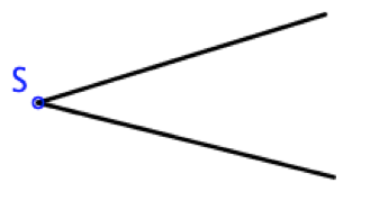
\includegraphics[scale=0.4]{images/Def-Winkel.png}
		\end{minipage}
	\end{definition}
	\begin{notation}
		Winkel werden mit den griechischen Kleinbuchstaben bezeichnet.
		\begin{enumerate}[label=\ ]\begin{multicols}{3}
				\item $\alpha\quad$ Alpha
				\item $\beta\quad$ Beta
				\item $\gamma\quad$ Gamma
				\item $\delta\quad$ Delta
				\item $\epsilon\quad$ Epsilon
				\item $\ldots$
		\end{multicols}\end{enumerate}
	\end{notation}
	Die Grösse eines Winkel kann mithilfe des Geodreiecks bestimmt werden. Dabei bezeichnen wir unterschiedlich grosse Winkel wie folgt:
	\begin{table}[H]
		\centering
		\begin{tabular}{m{4cm} m{4cm} m{7cm}}
			spitzer Winkel & 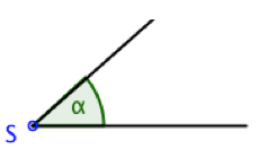
\includegraphics[width=3cm]{images/spitzerWinkel.png} & wenn $\alpha$ zwischen $0^\circ$ und $90^\circ$\\
			rechter Winkel & 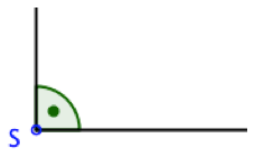
\includegraphics[width=3cm]{images/rechterWinkel.png} & wenn $\alpha=90^\circ$\\
			stumpfer Winkel & 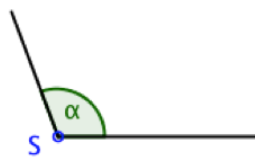
\includegraphics[width=3cm]{images/stumpferWinkel.png} & wenn $\alpha$ zwischen $90^\circ$ und $180^\circ$\\
			gestreckter Winkel & 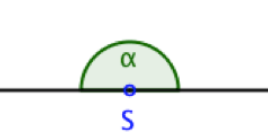
\includegraphics[width=3cm]{images/gestreckterWinkel.png} & wenn $\alpha=180^\circ$\\
			überstumpfer Winkel & 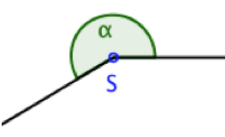
\includegraphics[width=3cm]{images/überstumpferWinnkel.png} & wenn $\alpha$ zwischen $180^\circ$ und $360^\circ$\\
		\end{tabular}
	\end{table}
	Falls wir mehrere Winkel miteinander vergleichen möchten, können wir für zwei sich schneidende Geraden folgenden Satz formulieren.
	\begin{satz}[Neben- und Scheitelwinkel]
		\begin{minipage}{0.6\linewidth}
			Winkel, die sich bei einer Geradenkreuzung nebeneinander befinden, heissen \textbf{Nebenwinkel}. Winkel, die sich bei einer Geradenkreuzung gegenüber befinden, heissen \textbf{Scheitelwinkel}. Für diese beiden Winkel gelten folgende Aussagen:
			\begin{enumerate}
				\item Die Summe zweier Nebenwinkel beträgt $180^\circ$.
				\item Scheitelwinkel sind gleich gross.
			\end{enumerate}
		\end{minipage}
		\hfill
		\begin{minipage}{0.35\linewidth}
			\centering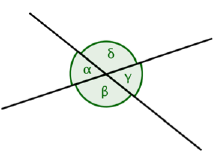
\includegraphics[scale=0.7]{images/scheitelwinkel.png}
		\end{minipage}
	\end{satz}
	Auf der anderen Seite können wir für zwei parallele Geraden ebenfalls einen Satz formulieren.
	\begin{satz}[Stufen- und Wechselwinkel]
		Für \textbf{Stufen-} und \textbf{Wechselwinkel}, die in der untenstehenden Grafik veranschaulicht werden, gilt folgende Aussage:
		\begin{center}
			\begin{figure}[H]
				\centering
				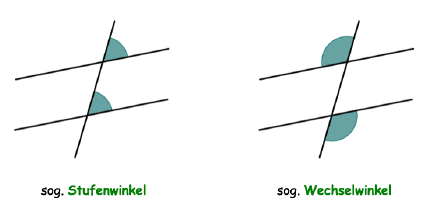
\includegraphics[scale=0.7]{images/stufenwinkel.png}
			\end{figure}
			Stufen- und Wechselwinkel sind gleich gross.
		\end{center}
	\end{satz}\newpage



\section{Winkelsätze bei Figuren}
	Vermutlich kennt ihr alle bereits die Winkelsumme eines Dreiecks. Jedoch habt ihr die Aussage wohl kaum riguros bewiesen. Da das Beweisen auch als Königsdisziplin der Mathematik betrachtet wird, möchte ich diese Aussage beispielhaft beweisen.
	\begin{satz}[Winkelsumme im Dreieck]
		In jedem Dreieck gilt: $\alpha+\beta+\gamma=180^\circ$.
	\end{satz}
	\begin{beweis}
		\karos{3.5}
	\end{beweis}
	Lasst uns die Winkelsumme für ein beliebiges Vieleck untersuchen.
	\begin{aufgabe}
		\begin{enumerate}[label=\alph*)]
			\item Dazu starten wir bei einem Viereck und zerlegen dieses in zwei Dreiecke, indem wir eine Diagonale einzeichnen. Zeichne eine Skizze und gib die Winkelsumme eines Vierecks an.
		\end{enumerate}
		\karos{4}
		\begin{enumerate}[label=\alph*)]\setcounter{enumi}{1}
			\item Und im Fünfeck? Zeichne auch hier verschiedene Möglichkeiten, um das Fünfeck in Dreiecke zu unterteilen und berechne die Winkelsumme.
		\end{enumerate}
		\karos{4}
		\begin{enumerate}[label=\alph*)]\setcounter{enumi}{2}
			\item Und im Siebeneck? Zeichne auch hier verschiedene Möglichkeiten, um das Siebeneck in Dreiecke zu unterteilen und berechne die Winkelsumme.
		\end{enumerate}
		\karos{4}
		\begin{enumerate}[label=\alph*)]\setcounter{enumi}{3}
			\item Zusammenfassend stelle eine Formel auf, die die Winkelsumme eines Vielecks in Abhängigkeit der Anzahl Eckpunkten $n$ berechnet.
		\end{enumerate}
		\karos{2}
	\end{aufgabe}
	\begin{satz}[Winkelsumme im $n-$Eck]
		Die Winkelsumme eines $n-$Eck lässt sich mit der folgenden Formel berechnen:\[\gap{5}.\]
	\end{satz}
	\begin{aufgabe}
		Löse die Aufgaben zur Winkelberechnungen.
	\end{aufgabe}\newpage



\section{Der Satz des Thales}
	\begin{minipage}{0.6\linewidth}
		Wir betrachten einen Halbkreis mit gegebenem Durchmesser $\overline{AB}$. Irgendwo auf dem Halbkreis wählen wir einen weiteren Punkt $C$.\vspace{11pt}\newline
		Da $\overline{AM}=\overline{BM}=\overline{CM}$ (Radius des Halbkreis), sind die Dreiecke $\triangle AMC$ und $\triangle BMC$ gleichschenklig und haben also jeweils zwei gleich grosse Winkel.
	\end{minipage}
	\hfill
	\begin{minipage}{0.35\linewidth}
		\centering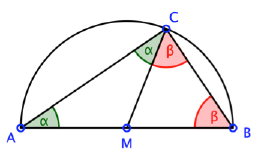
\includegraphics[scale=0.7]{images/thaleskreis.png}
	\end{minipage}\vspace{5pt}
	Das grosse Dreieck $\triangle ABC$ hat wie jedes andere Dreieck eine Winkelsumme von $180^\circ$. Das heisst:
	\vspace{2.4cm}\newline
	Das bedeutet also, unser Dreieck $\triangle ABC$ ist - unabhängig von der Position von $C$ auf dem Halbkreis - rechtwinklig mit einem rechten Winkel beim Eckpunkt $C$.
	\begin{satz}[Satz des Thales]
		Liegt der Punkt $C$ eines Dreiecks $\triangle ABC$ auf dem Halbkreis über der Strecke $\overline{AB}$, dann hat das Dreieck bei $C$ einen rechten Winkel.
	\end{satz}
	\begin{aufgabe}
		Löse die Aufgaben zu den Winkelberechnungen mithilfe des Thaleskreises.
	\end{aufgabe}\newpage



\section{Der Peripherie- und Zentriwinkelsatz}
	In der folgenden Aufgabe möchten wir den Zentriwinkelsatz beweisen. Bevor wir aber starten, möchten wir die Begriffe Peripherie- und Zentriwinkel zuerst definieren.
	\begin{definition}
		Der Winkel \gap{3} heisst \textbf{Zentriwinkel} und der Winkel \gap{3} heisst \textbf{Peripheriewinkel} über der Sehne $\overline{AB}$.
	\end{definition}
	\begin{figure}[H]
		\centering
		\begin{tikzpicture}[cross/.style={draw, cross out, minimum size=2*(#1-1pt), inner sep=0pt, outer sep=0pt}, x=1cm, y=1cm,
			>=latex,   %Voreinstellung für Pfeilspitzen
			font= \footnotesize, scale=0.6]
			\draw[black, very thick](-1,0) circle (5);
			\filldraw[black] (-1,0) circle (2pt) node[anchor=east]{$M$};
			\filldraw[black] (4,0) circle (2pt) node[anchor=west]{$B$};
			\filldraw[black] (-5,-3) circle (2pt) node[anchor=east]{$A$};
			\filldraw[black] (-1,5) circle (2pt) node[anchor=south]{$P$};
			\draw[black,very thick] (-5,-3) -- (4,0);
			\draw[black,very thick] (-5,-3) -- (-1,0);
			\draw[black,very thick] (-1,0) -- (4,0);
			\draw[black,very thick] (4,0) -- (-1,5);
			\draw[black,very thick] (-5,-3) -- (-1,5);
		\end{tikzpicture}
	\end{figure}
	\begin{aufgabe}
		Betrachte das folgende \href{https://www.geogebra.org/m/exmt29g4}{Geogebra-Applet}, in dem die beiden Punkte $A$ und $P$ verschoben werden können. Stelle basierend auf deinen Beobachtungen eine Behauptung auf, in der beide Winkel $\mu$ und $\phi$ vorkommen. \[\gap{1}\*\mu=\gap{1}\*\phi\]
		Nun möchten wir deine Behauptung auch beweisen.
		\begin{enumerate}
			\item Zeichne die Strecke $\overline{MP}$ ein.
			\item Stelle eine Formel für die Berechnung der Winkelsumme des Dreiecks $\triangle AMB$ und des Dreiecks $\triangle APB$ auf.
			\begin{align*}
				180^\circ &= \gap{5}\\
				180^\circ &= \gap{5}
			\end{align*}
			\item Da die linke Seite der beiden obigen Formel gleich sind, können die beiden rechten Seiten gleichgesetzt werden. \[\gap{5}=\gap{5}\] Forme die entstandene Gleichung nun soweit um, bis du deine Behauptung findest.
		\end{enumerate}
		\karos{4}
		Damit haben wir den Zentriwinkelsatz erfolgreich bewiesen.
	\end{aufgabe}
	\begin{satz}[Zentriwinkelsatz]
		Der Zentriwinkel $\mu$ über einer Sehne $\overline{AB}$ ist genau doppelt so gross wie der zugehörige Peripheriewinkel $\phi$.
	\end{satz}
	Analog zum Zentriwinkelsatz können wir mithilfe des Geogebra-Applets auch noch den Peripheriewinkelsatz behaupten. Wir verzichten aber hier ausnahmsweise auf einen detailierten Beweis. Der Peripheriewinkelsatz besagt also folgendes:
	\begin{satz}[Peripheriewinkelsatz]
		Alle Peripheriewinkel $\phi$ über der gleichen Sehne $\overline{AB}$ sind gleich gross; i.e. Der Punkt $P$ kann frei verschoben werden, ohne dass sich der Winkel verändert.
	\end{satz}
	\begin{aufgabe}
		Löse die Aufgaben zum Peripherie- und Zentriwinkelsatz.
	\end{aufgabe}


\newpage
\subsection*{History}
\begin{table}[H]
	\centering
	\begin{tabular}{|p{13mm}|p{20mm}|p{30mm}|p{70mm}|}\hline
		%\multicolumn{4}{|l|}{History}\\\hline
		Version & Datum & Person & Bemerkung \\\hline
		$1.0$ & 14.09.2024 & Jonas Guler & Kapitel erstellt \\\hline
		$1.1$ & ToDo & Jonas Guler & Aufgaben zusammensuchen \\\hline
	\end{tabular}
\end{table}


\end{document}